\chapter{Research Design and Methodology}
\label{chap:methodology} This chapter details the methodology employed to achieve
the primary objective of this study: extending the explainability of path-based
knowledge graph recommender systems to explore "what-if" scenarios.

The methodology is structured as follows:
\begin{enumerate}
	\item \textbf{Initial Recommendation}: The process initiates with the system generating
	      a product recommendation for a user. In a path-based recommendation system, the
	      inherent explanation typically comprises a sequence of entities and relationships
	      that link the user to the recommended product.

	\item \textbf{Counterfactual Analysis}:
	      \begin{itemize}
		      \item \textbf{Extraction of Relevant Information}:
		            Relevant attributes for the counterfactual analysis are those that could
		            potentially be associated with the entity under examination. By analyzing these attributes,
		            we gain insights into the recommendations for the final product. The process of extracting
		            relevant information begins with the removal of outlier nodes in the knowledge graph,
		            using centrality measures to identify these nodes. Based on the nodes along the path,
		            the recommended product, and connected entities, we select potential relevant
		            attributes. These attributes are then further refined by considering the communities
		            identified within the graph.

		      \item \textbf{Scenario Construction}: Utilizing the extracted information,
		            a collection of hypothetical scenarios is constructed. These scenarios are
		            crafted to test various alterations in attributes and their impact on the
		            recommendation outcome.
	      \end{itemize}

	\item \textbf{Recommendation System Utilization}: For the recommendation engine,
	      we employ CAFE (Coarse-to-Fine Neural Symbolic Reasoning for Explainable Recommendation).
	      This system is particularly suitable for our purposes due to its path-based nature
	      and its capability to evaluate the plausibility of different paths by assigning
	      probability scores to the steps that connect users to products.
\end{enumerate}
\vspace{12pt}
This methodology both facilitates a deeper understanding of the decision-making processes
inherent in the recommender system and also allows us to simulate and evaluate how
changes in product attributes or user-product relationships might alter the system's
recommendations.

\section{Recommender System Details}
%TODO add citation
CAFE (Coarse-to-Fine Neural Symbolic Reasoning for Explainable Recommendation)
serves as the foundational framework for our path-based knowledge graph
recommender system. This framework is particularly suited to our needs because it
allows for detailed access to the scores of each path within the graph,
facilitating the analysis of the counterfactual scenarios. This section provides
an overview of its implementation and core functionalities.

\subsection{Data and Implementation}
The CAFE model is implemented using the Amazon review dataset, the beauty
category, which includes comprehensive user and product interactions. It
leverages predefined embeddings train in the model developed by \textcite{ai_learning_2018} described
in the previous section, as input to their symbolic network.
\subsection{Knowledge Graph Composition}
The knowledge graph at the heart of this recommendation system is intricately structured,
comprising several types of entities and relationships:
\begin{itemize}
	\item \textbf{Users} are linked to the products
	      they have purchased and the words they have used.

	\item \textbf{Products} are associated with descriptive words, their brand,
	      category, and other related products. Relationships with related products
	      include those that have been 'bought together', 'also viewed', and 'also bought'.

	\item \textbf{Brands and Categories} form additional nodes, creating multiple pathways
	      that connect different aspects of the data.

	\item \textbf{Related Products} mentioned above.
\end{itemize}
\begin{figure}[h!]
	\begin{center}
		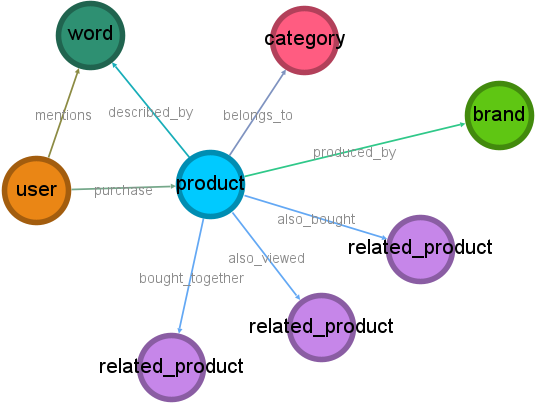
\includegraphics[width=0.6\columnwidth, keepaspectratio]{images/knowledge_graph_structure.png}
		\caption{Knowledge Graph Nodes and Relations Types}
		\label{fig:knowledge_graph_structure}
	\end{center}
\end{figure}
The enitity types and the relationships between the nodes are demonstrated in
\fref{fig:knowledge_graph_structure}.

\subsection{Path-Based Recommendation Mechanics}
The system operates on predefined metapaths that represent meaningful
relationships leading a user to a product. These metapaths outline the possible structure
of paths that could lead a user to purchase a product.
\begin{figure}[h!]
	\begin{center}
		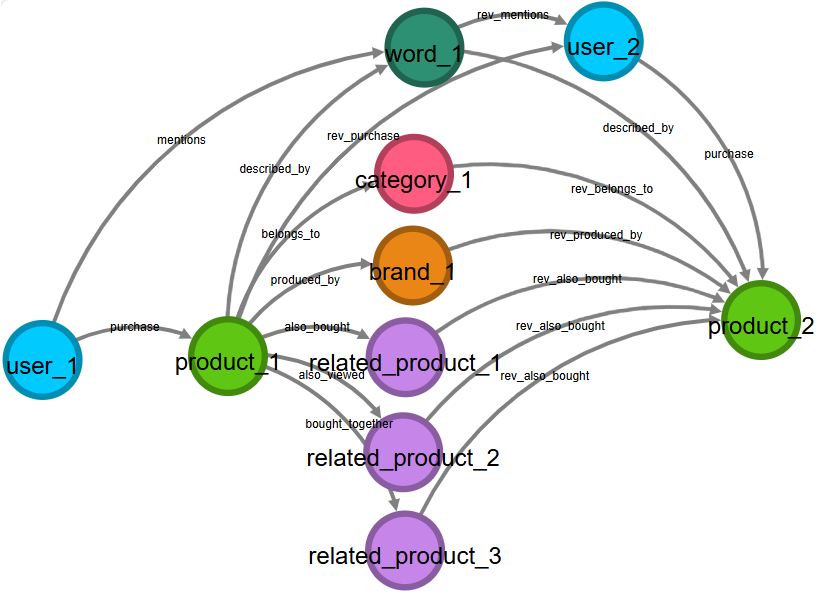
\includegraphics[width=0.9\columnwidth, keepaspectratio]{
			images/metapaths.png
		}
		\caption{Metapaths Definded Within Recommender Systsm}
		\label{fig:metapaths}
	\end{center}
\end{figure}
The structures of metapaths used in the recommeder system at hand are domenstrated
in \fref{fig:metapaths}.

The recommender system assigns a probability score to each step along the path, determining
the strength of the connection between the user and the potential product recommendations.
It then selects the top 10 paths with the highest cumulative scores, and the products
associated with these paths are recommended to the user. This scoring and
selection process ensures that the recommendations are both relevant and
tailored to the user's preferences and behavior patterns. This structured approach
allows the CAFE system to effectively recommend products and offer insights into
the reasons behind each recommendation, enhancing the system's explainability.

\section{Counterfactual Analysis}
Following the predictions provided by the recommender system, for the counterfactual
analsyis of the recommended product, a threshold is determined for the minimum
score required for a product path to be recommended to a user. This threshold corresponds
to the path score of the last product in the top 10 recommended products.

The next step involves retreiving the first-level products related to the
attributes of the recommended product, and through them, extraction of possible
relevant attributes. This forms the initial layer of attribute selection,
grounded on the hypothesis that first-level connected items possess possiblly
relevant attributes. These relevent attributes, after undergoing refinement and filitering processes, 
make up the counterfactual scnenarios to be analyzed for plausability. 

Since the scoreing of attributes is based on the metapaths defined in the system,
after the selection of relevant attributes, an appropriate metapath is selected
based on the type of the attribute. Using the recommender engine, we calculate
the score for user-product combinations, which incorporates all the products previously
purchased by the user and the counterfactual attribute in question. If the
recalculated score for a product, involving the counterfactual attribute,
exceeds the determined minimum score, the attribute is considered a positive influence
for a product similar to the recommended one.

This isolated attribute analysis aids in understanding the influence of specific
attributes on product recommendations and also provides marketing insights. Such
insights can further be used to enhance the diversity and precision of the recommender
system.

\section{Attribute Filtering and Knowledge Graph Refinement}
To select the most relevant counterfactual attributes for the product under
analysis and ensure they add value to our study, we eliminate outlier nodes from
the knowledge graph. Additionally, we conduct community detection to restrict attribute
selection to those within the same community as the product being analyzed.

\subsection{Outlier Nodes Detection and Removal}
For the purpose of the oulier detection and removal, we use the degree centrality
of nodes in the knowledge graph. Nodes that exhibit a degree centrality above a
certain threshold are eliminated. While these highly connected nodes can provide
valuable insights for counterfactual analysis, they often include unhelpful
elements such as universally common categories or frequently used words that
lack distinctive features. Additionally, since they disrupt the modularity of
communities essential for selecting relevant attributes, these nodes are removed.

\subsubsection*{Degree Centrality of Nodes}
For a given node, degree centrality is the number of edges connected to that node
\parencite{bloch2023centrality}

The use of degree centrality is justified given the structure of the knowledge
graph, where node types such as category, brand, and related products are connected
exclusively to product nodes, as shown in Figure \ref{fig:knowledge_graph_structure}. This measure will determine
how many products each of these attribute nodes is connected to, which will help
in deciding whether to retain or remove them as outliers based on a
predetermined threshold. For word attributes, however, since word nodes are connected
not only to product nodes but also to user nodes, we apply a modified approach. Rather
than using degree centrality, we count only the connections between each word
node and product nodes.

\begin{figure}[h!]
	\begin{center}
		% 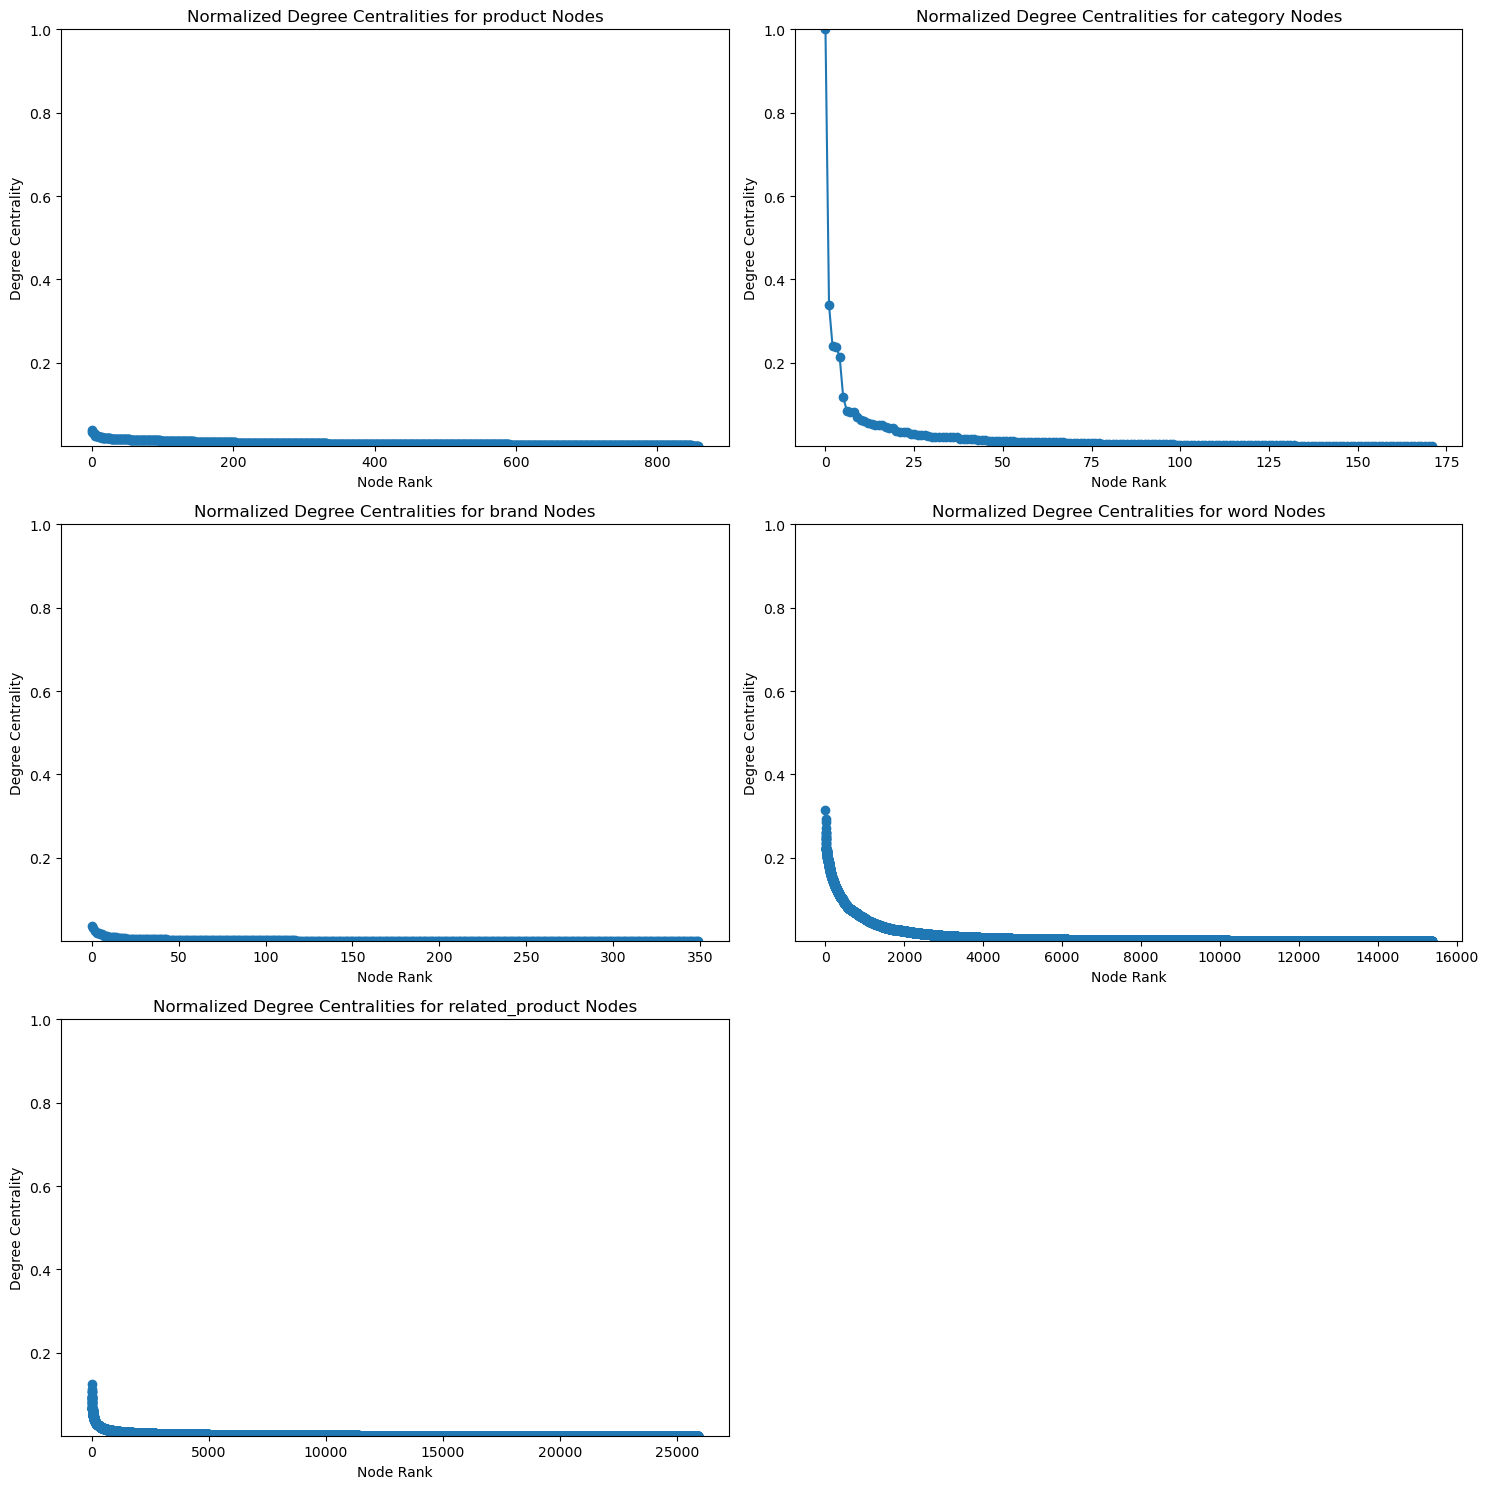
\includegraphics[width=0.6\columnwidth, keepaspectratio]{images/degree_centrality_distributions_by_node_type.png}
		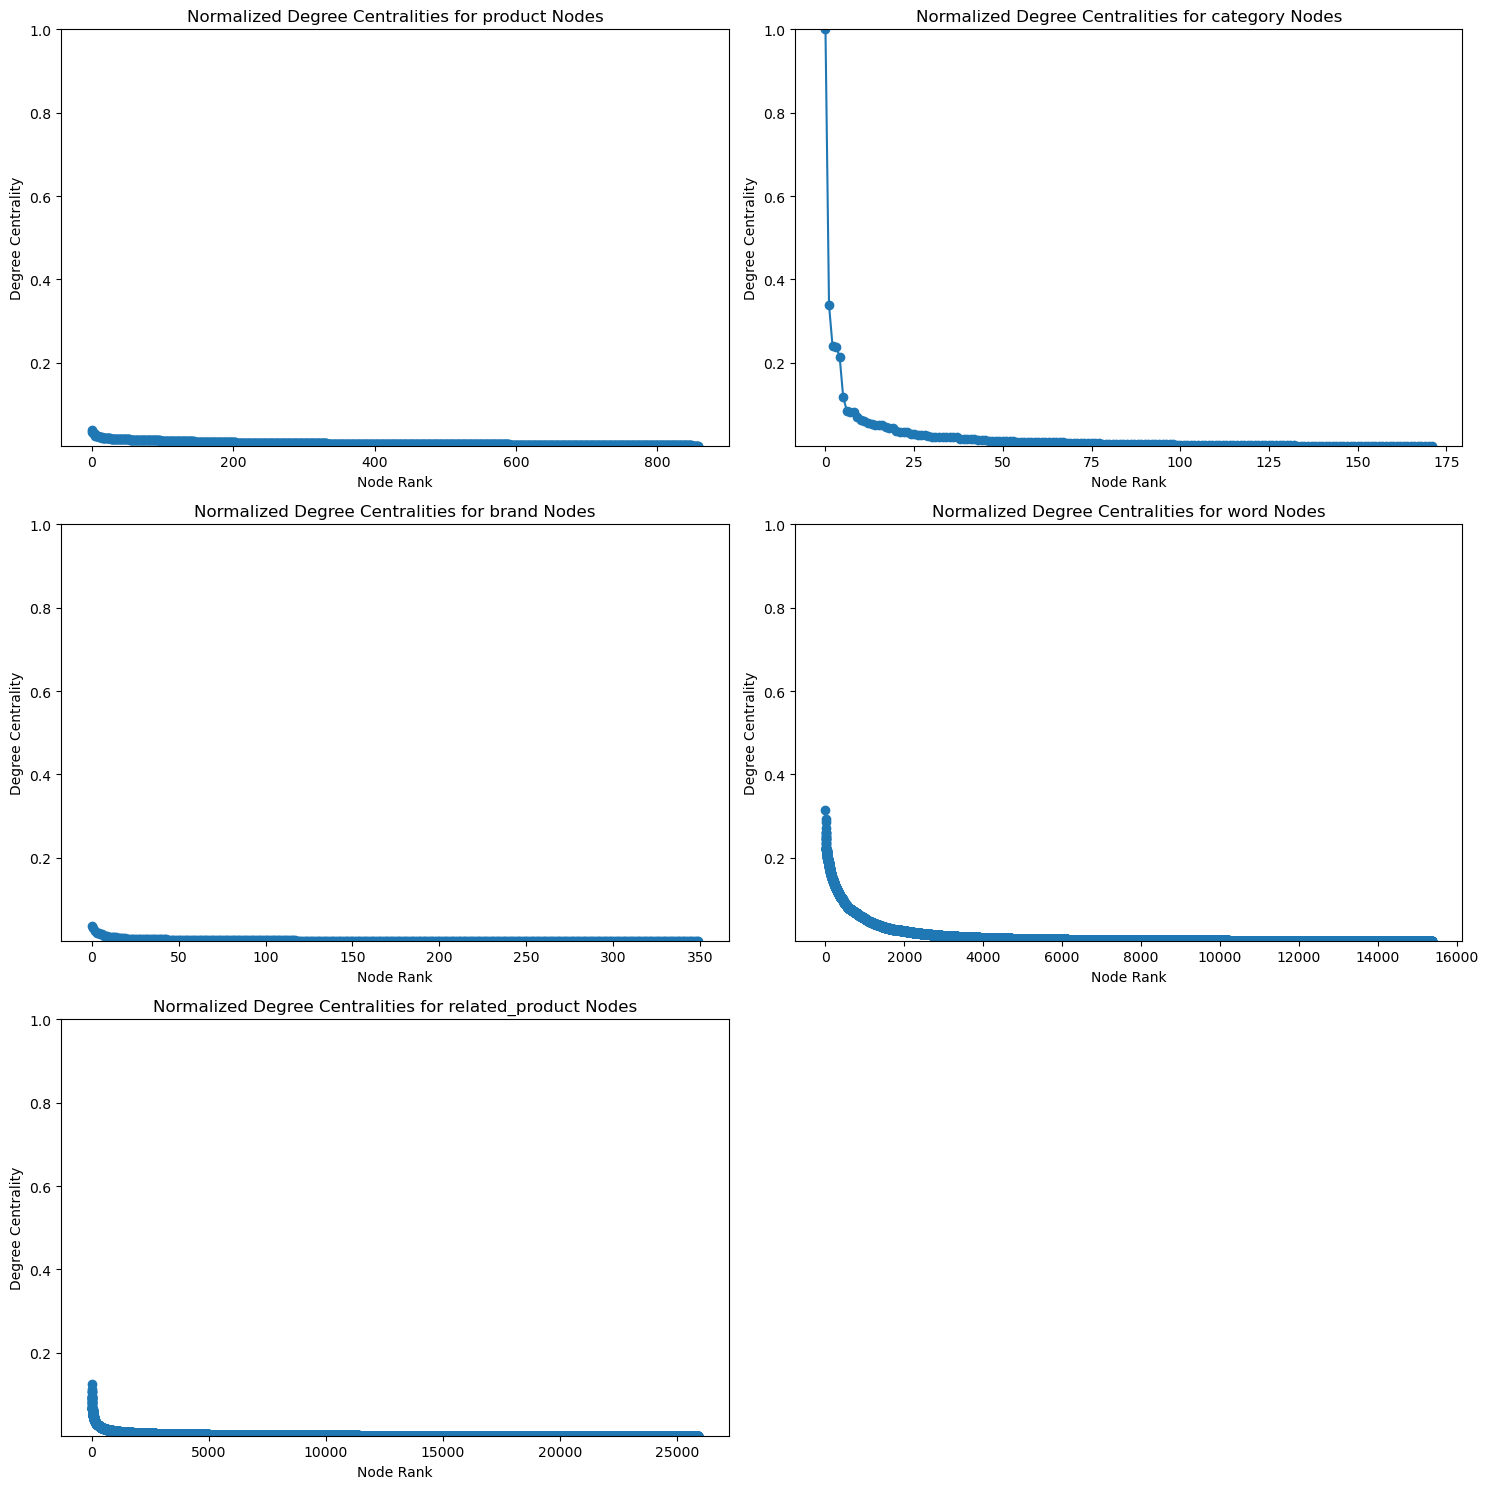
\includegraphics[width=\columnwidth, keepaspectratio=true]{images/degree_centrality_distributions_by_node_type.png}
		\caption{Degree Centrality Distributions of Nodes by Node Type}
		\label{fig:degree_centrality_distributions_by_node_type}
	\end{center}
\end{figure}
The degree centrality of different types of nodes are demonstrated in \fref{fig:degree_centrality_distributions_by_node_type}.
It is apparent from the plots that some nodes have unusual degree centralities.

\subsubsection*{Determining The Outlier Nodes}

Based on the reasons described, it was necessary to remove the outlier nodes while
retaining the structure of the original knowledge graph as much as possible.
Various statistical methods for outlier detection were experimented with, and the
method that removed the least number of nodes while maintaining the highest community
resemblance was chosen. Specifically, the knee method was used to identify and remove
the outlier nodes.

\subsubsection*{Knee Detection}
For the detection of the knee in the degree centrality of nodes, the Kneedle algorithm
have been used. The Kneedle algorithm identifies "knee points" in data, which represent
the points where the rate of improvement in performance begins to level off significantly
in relation to changes in a tunable system parameter, degree centrality in our
case. It operates by first calculating a difference curve from normalized data points,
highlighting the deviations from a direct diagonal line. The algorithm then detects
local maxima in this difference curve, pinpointing where the rate of change in
the response variable starts to decrease sharply, indicating the presence of a knee
\parencite{satopaa_finding_2011}.

In \fref{fig:degree_centralitites_and_knee_point} the degree centralities of all
nodes with different types are represented in a plot, arranged in decreasing order. The Kneedle
algorithm is used to detect the knee point in the values of degree centralities.
This knee point marks a transition where the differences in degree centrality
become less significant beyond this point compared to those before it.



\begin{figure}[h!]
	\begin{center}
		% 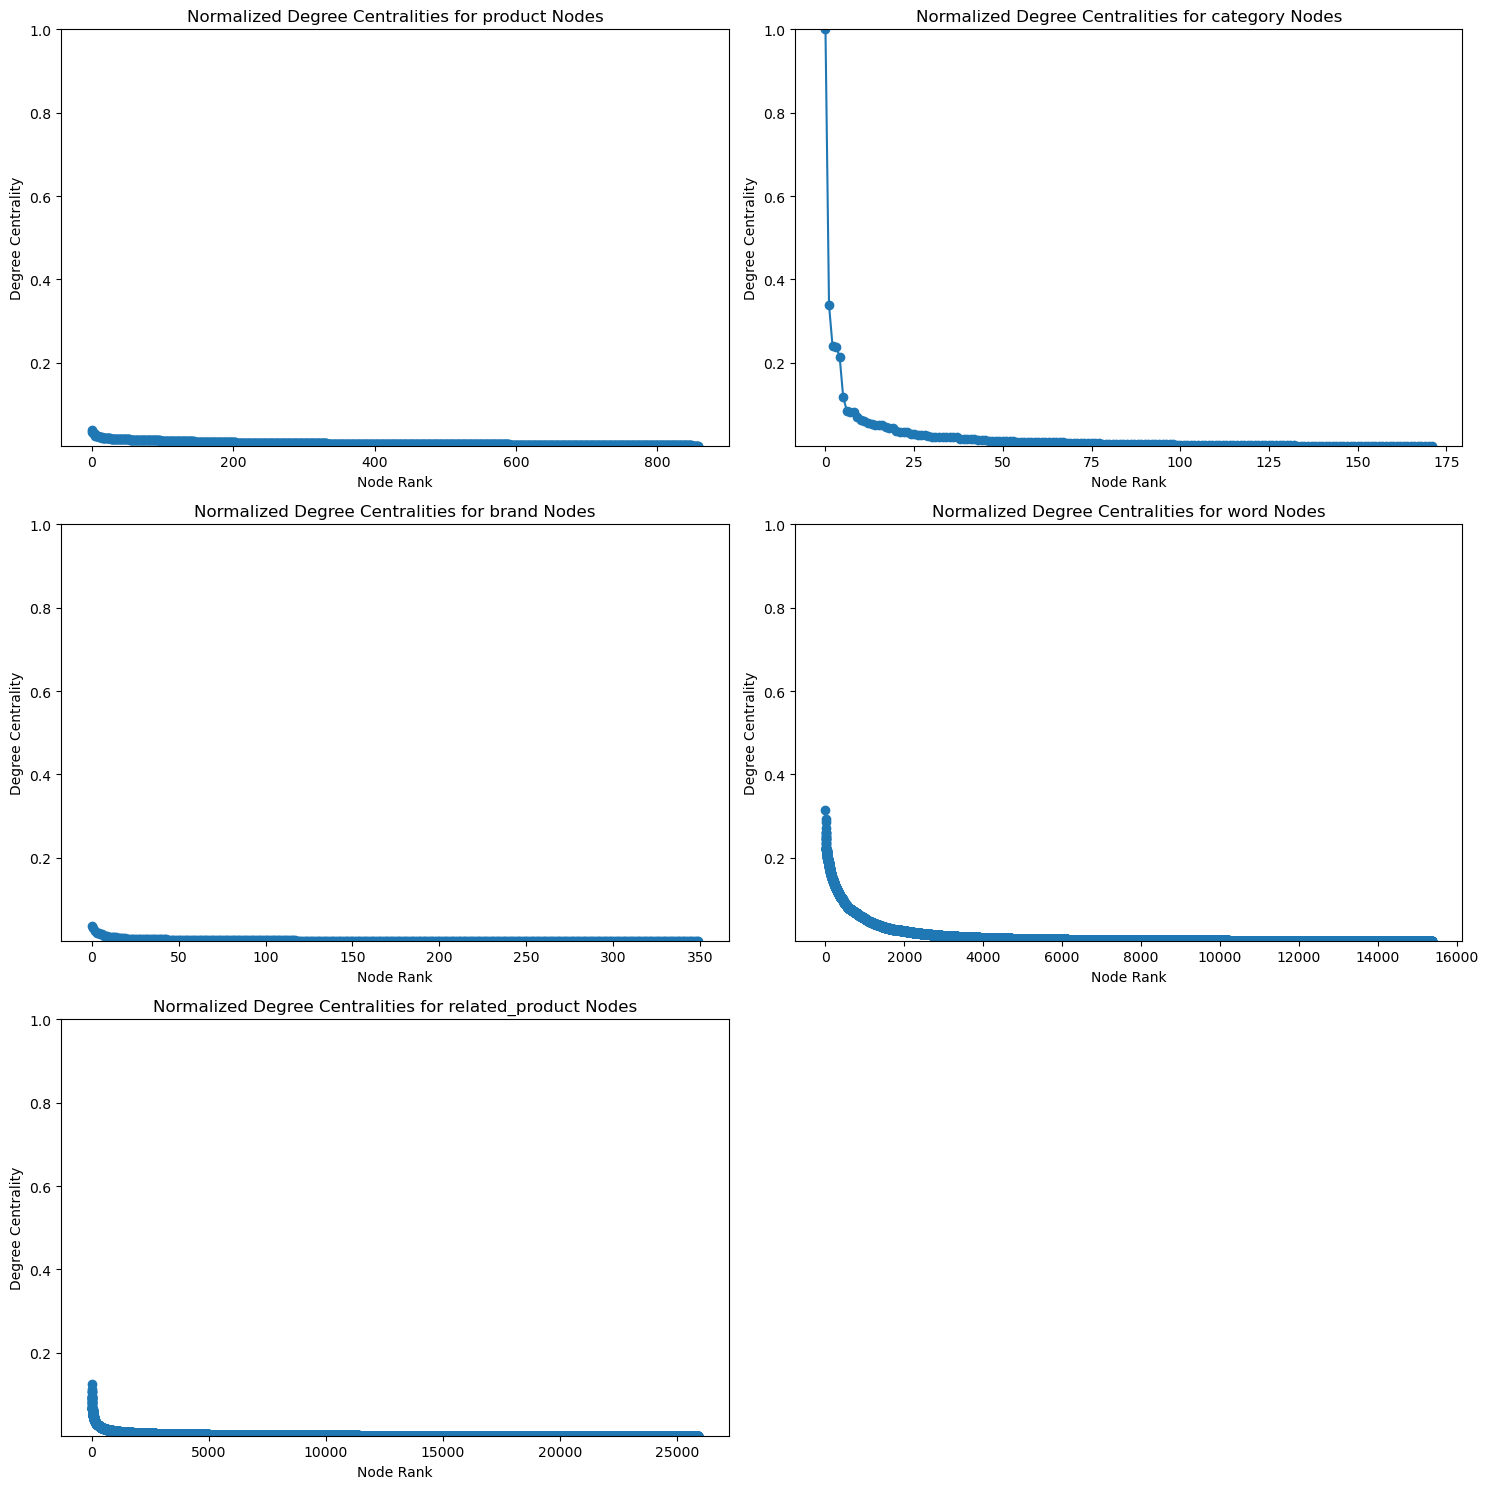
\includegraphics[width=0.6\columnwidth, keepaspectratio]{images/degree_centrality_distributions_by_node_type.png}
		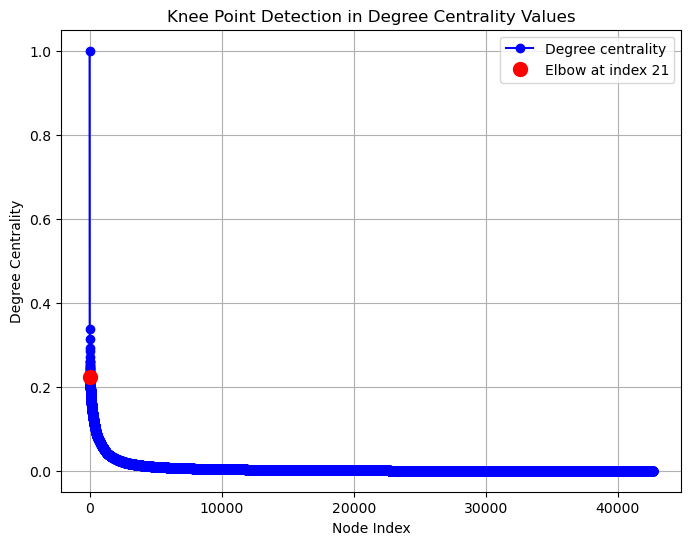
\includegraphics[width=\columnwidth, keepaspectratio=true]{images/degree_centralitites_and_knee_point.png}
		\caption{Degree Centrality of All Nodes and Knee Point Specified with Kneedle Algorithm}
		\label{fig:degree_centralitites_and_knee_point}
	\end{center}
\end{figure}

In \fref{tab:graph_metrics} the number of nodes removed and consequent changes are represented.

\begin{table}[h]
	\centering
	\begin{tabular}{l c}
	\hline
	\textbf{Metric} & \textbf{Value} \\
	\hline
	Nodes Removed & 25 \\
	Number of Communities in Original Graph & 22 \\
	Number of Communities in Cleaned Graph & 24 \\
	Number of Nodes in the Original Graph & 42670 \\
	Number of Nodes in the Cleaned Graph & 42645 \\
	\hline
	\end{tabular}
	\caption{Graph Metrics Before and After Cleaning}
	\label{tab:graph_metrics}
	\end{table}


\subsection{Community Detection and Graph Analysis Node Filtering}
The next step in the counterfactual analysis is the detection of communities within the knowledge graph of interactions.
Communities are identified using Louvain Method. This helps to cluster entities that
share significant similarities and interactions. The Louvain Method is a an
efficient algorithm designed for detecting communities in large-scale networks
by optimizing modularity, a measure that quantifies the density of links within communities
relative to those between them introduced in \parencite{blondel_fast_2008}. 

In the case of weighted networks the
modularity $Q$ is defined as:

\begin{equation}
	\label{eq:modularity}Q = \frac{1}{2m}\sum_{i,j}\left[ A_{ij}- \frac{k_{i} k_{j}}{2m}
	\right] \delta(c_{i}, c_{j}),
\end{equation}

where $A_{ij}$ represents the weight of the edge between nodes $i$ and $j$,
$k_{i} = \sum_{j}A_{ij}$ is the sum of the weights of the edges attached to
vertex $i$, and $c_{i}$ is the community to which vertex $i$ is assigned. The
$\delta$-function $\delta(c_{i}, c_{j})$ equals 1 if $c_{i} = c_{j}$ and 0
otherwise. Here, $m = \frac{1}{2}\sum_{ij}A_{ij}$ represents the sum of the
weights of all the edges in the network. In the case of unweighted networks,
where no specific weights are assigned to the edges, each edge is assumed to have
a weight of 1.

The change in modularity $\Delta Q$ when moving a node $i$ to a different
community is given by:

\begin{equation}
	\label{eq:delta_modularity}\Delta Q = \left[ \frac{\sum_{\text{in}}+ k_{i, \text{in}}}{2m}
	- \left( \frac{\sum_{\text{tot}}+ k_{i}}{2m}\right)^{2}\right] - \left[ \frac{\sum_{\text{in}}}{2m}
	- \left( \frac{\sum_{\text{tot}}}{2m}\right)^{2}- \left( \frac{k_{i}}{2m}\right
	)^{2}\right],
\end{equation}

where $\sum_{\text{in}}$ is the sum of the weights of the edges inside the community,
$k_{i, \text{in}}$ is the sum of the weights of the edges from node $i$ to other
nodes in the community, and $\sum_{\text{tot}}$ is the total sum of the weights of
the edges to nodes in the community. $k_{i}$ represents the degree of node $i$, which
is the sum of the weights of all edges attached to node $i$. If the network is
unweighted, the weight $A_{ij}$ is taken to be 1 for all edges.

The algorithm operates in two iterative phases: initially, it optimizes modularity
locally, evaluating potential gains by moving individual nodes into different
communities. Nodes are shifted to the community that maximizes this gain, and
the process is repeated until no further improvement is possible, achieving a local
maximum of modularity. In the second phase, the method aggregates these identified
communities into new nodes of a reduced network, and the process is reapplied. This
hierarchical approach allows the algorithm to uncover community structures at multiple
levels effectively. Notable for its speed, the Louvain Method can handle networks
with up to millions of nodes efficiently, making it well-suited for modern
datasets of substantial size. To refine the analysis further, we calculate the
degree centrality for each type of pair within the graph. Nodes that do not provide
significant insight are filtered out based on their z-score; specifically, nodes
with a z-score exceeding [specific threshold] are removed.


\subsection{Attribute Selection}
Following the predictions provided by the recommender system, a threshold is determined
for the minimum score required for a product path to be recommended to a user.
This threshold corresponds to the path score of the last product in the top 10
recommended products.
For the analysis of a recommended path, we retrieve the first-level attributes and
their related products. This forms the initial layer of attribute selection, predicated
on the hypothesis that first-level connected items possess more relevant attributes.
These selected attributes are then evaluated to determine whether they fall
within the community of the recommended product. If they do, and their z-score
is within an acceptable range, they are considered for further counterfactual analysis.



\section{Case Study}